% =====================================================================
%  Passaggio al limite sotto il segno di integrale -- lezione 2
% =====================================================================

% [0:56:36]
\section{Passaggio al limite sotto il segno di integrale}

\subsection{Il problema}

Data una successione $f_n\colon[a,b]\to\mathbb{R}$ con limite $f$, ci si chiede se
\[
\int_a^b \Big(\lim_{n\to\infty} f_n(x)\Big)\,dx
\;=\;
\lim_{n\to\infty}\int_a^b f_n(x)\,dx .
\]
L'interesse pratico è evidente: a sinistra si integra la funzione limite, che di
solito è molto più semplice; a destra si integra ciascuna $f_n$ e poi si passa al
limite. Poterle scambiare significa poter approssimare un integrale difficile con una
successione di integrali facili.

\subsection{Enunciato}

\Teorema{passaggio al limite sotto il segno di integrale}{%
Siano
\begin{enumerate}
  \item $f_n\colon[a,b]\to\mathbb{R}$ continua per ogni $n$;
  \item $f_n\rightrightarrows f$ in $[a,b]$.
\end{enumerate}
Allora
\begin{equation}
\lim_{n\to\infty}\int_a^b f_n(x)\,dx
=\int_a^b \lim_{n\to\infty} f_n(x)\,dx
=\int_a^b f(x)\,dx .
\end{equation}
}

\BoxBlue{Osservazione}{}{%
Il limite $f$ che compare a destra è il limite puntuale
della successione; per il teorema di continuità del limite $f$ è continua, quindi
tutti gli integrali scritti hanno senso. Si noti anche che, mentre a sinistra si ha
una successione \emph{numerica} $I_n=\int_a^b f_n$, l'ipotesi di convergenza richiesta
sulle funzioni è quella uniforme: l'integrale definito è un numero, ma per controllarlo
serve un'informazione valida su tutto $[a,b]$ contemporaneamente.
}

\BoxBlue{Osservazione}{}{%
L'implicazione non si inverte: la validità del passaggio al
limite non garantisce la convergenza uniforme. Gli esempi che seguono chiariscono i
due lati della questione.
}

% [1:00:28]
\subsection{Due esempi}

\paragraph{Esempio 1.} $f_n(x)=n\,x\,(1-x^2)^n$, $x\in[0,1]$.

Limite puntuale: per $x=1$ si ha $f_n(1)=0$ per ogni $n$; per $0\le x<1$ la base
$1-x^2$ è minore di $1$, e l'esponenziale vince sulla potenza, quindi $f_n(x)\to 0$.
Dunque $f\equiv 0$ e
\[
\int_0^1 f(x)\,dx=0 .
\]
D'altra parte, riconoscendo a meno del fattore $-\tfrac{1}{2}$ la derivata di
$1-x^2$,
\[
\int_0^1 n\,x\,(1-x^2)^n\,dx
=-\frac{n}{2}\,\frac{(1-x^2)^{n+1}}{n+1}\bigg|_0^1
=0+\frac{n}{2(n+1)}
\;\xrightarrow[n\to\infty]{}\;\frac{1}{2}\neq 0 .
\]
Il passaggio al limite non vale, quindi per il teorema la convergenza \emph{non} può
essere uniforme (figura~\ref{fig:03}).

\begin{figure}[htbp]\centering
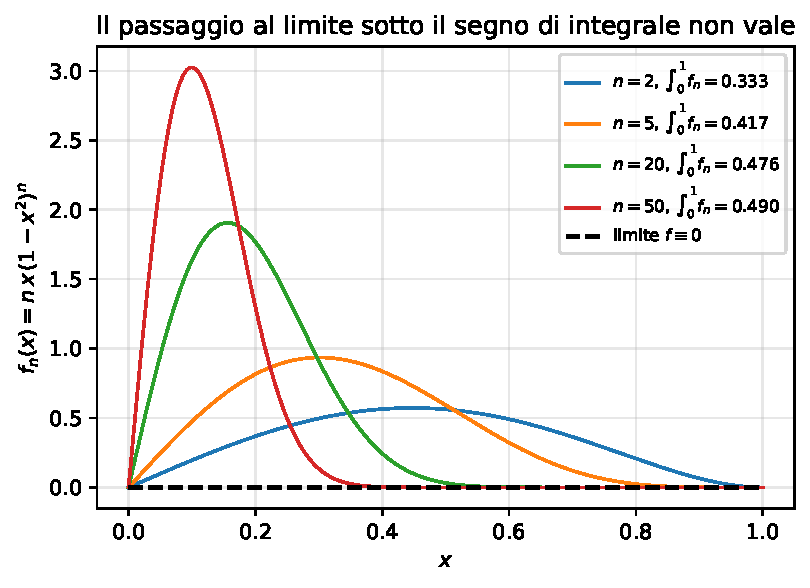
\includegraphics[width=0.6\linewidth]{figure/fig_03}
\caption{Andamento qualitativo di $f_n(x)=n\,x\,(1-x^2)^n$ su $[0,1]$: le funzioni
tendono puntualmente a zero, ma l'area sottesa tende a $1/2$.}
\label{fig:03}
\end{figure}

\paragraph{In aula.} Questo è il modo più economico di procedere: verificato che il
passaggio al limite fallisce, si conclude subito che la convergenza non è uniforme e
si evita completamente lo studio del $\sup$. (Per esercizio si può fare anche
direttamente: la derivata porta a una successione di massimi che non tende a zero.)

% [0:58:06]
\paragraph{Esempio 2.} $f_n(x)=n\,x\,e^{-nx}$, $x\in[0,1]$ (esercizio per casa, si
trova sul libro). Qui la convergenza è soltanto puntuale a $f\equiv 0$ — il massimo
vale $1/e$ per ogni $n$, raggiunto in $x=1/n$ — eppure il passaggio al limite vale,
perché $\int_0^1 f_n\to 0$ (figura~\ref{fig:04}).

\begin{figure}[htbp]\centering
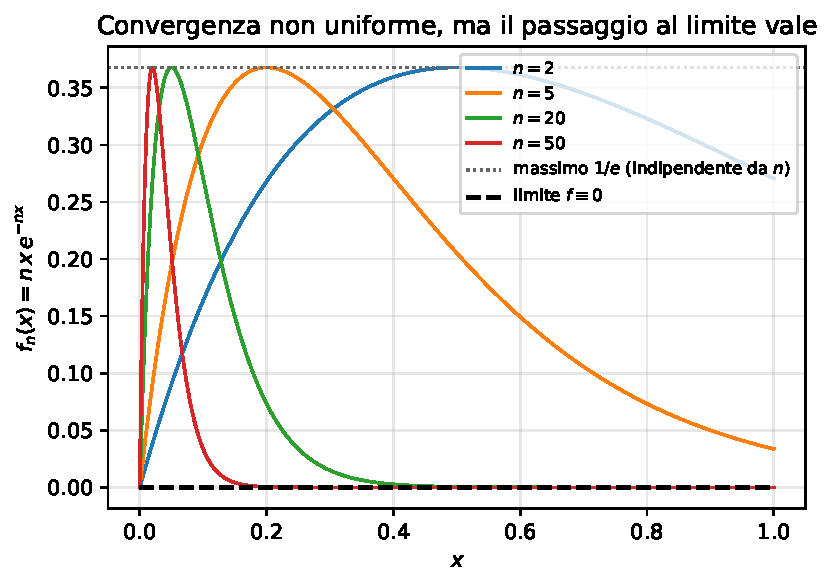
\includegraphics[width=0.6\linewidth]{figure/fig_04}
\caption{Andamento qualitativo di $f_n(x)=n\,x\,e^{-nx}$ su $[0,1]$: convergenza
puntuale non uniforme, ma gli integrali tendono comunque a zero.}
\label{fig:04}
\end{figure}

\BoxBlue{Osservazione}{}{%
I due esempi insieme dicono che: (i) la sola convergenza
puntuale, anche verso un limite ottimo (addirittura costante), non basta a garantire
il passaggio al limite; (ii) viceversa, il passaggio al limite può valere senza
convergenza uniforme, quindi l'implicazione del teorema non si inverte.
}

% [1:00:28]
\paragraph{In aula.} Le successioni $x^n$ e $x^{1/n}$ su $[0,1]$ non si prestano a
questo confronto: il loro limite è discontinuo in un estremo, e per evitarlo
bisognerebbe restringersi a $[0,a]$ con $a<1$, dove però la convergenza torna a essere
uniforme e non c'è più niente da osservare. L'esempio 1 è appunto una modifica di
$x^n$ costruita per aggirare questa difficoltà.

% [1:05:58]
\subsection{Dimostrazione}

Posto $I_n=\int_a^b f_n(x)\,dx$ e $I=\int_a^b f(x)\,dx$, si vuole mostrare che
$I_n\to I$: basta stimare $|I_n-I|$ con una quantità che tende a zero e concludere con
il teorema dei carabinieri. Si ha
\begin{align*}
|I_n-I|
&=\left|\int_a^b \big(f_n(x)-f(x)\big)\,dx\right|
&&\text{(linearità dell'integrale)}\\
&\le \int_a^b \big|f_n(x)-f(x)\big|\,dx
&&\text{(modulo dentro l'integrale)}\\
&\le \max_{x\in[a,b]}\big|f_n(x)-f(x)\big|\cdot(b-a)
&&\text{(confronto fra integrali)} .
\end{align*}
Il massimo esiste per il teorema di Weierstrass: la funzione $|f_n-f|$ è continua,
perché $f_n$ è continua per ipotesi e $f$ lo è per il teorema di continuità del limite.
Infine, per la convergenza uniforme, $\max_{[a,b]}|f_n-f|\to 0$, mentre $(b-a)$ è un
numero fissato: il prodotto tende a zero e, essendo $0\le|I_n-I|$, si conclude
$|I_n-I|\to 0$. $\blacksquare$

\paragraph{In aula.} Il passaggio con il massimo è quello che a scuola si chiama
``primo teorema della media'': in realtà è soltanto la proprietà di confronto fra
integrali, dato che la funzione è positiva e limitata superiormente dal suo massimo.
Al posto del massimo si può scrivere il $\sup$, che qui coincide.

% [1:10:49]
\paragraph{In aula.} La richiesta di convergenza uniforme è molto forte: moltissime
successioni convergono soltanto puntualmente e restano quindi fuori dal teorema. È
proprio questo il motivo per cui nel corso di Metodi verrà costruito un altro tipo di
integrale, con il quale il passaggio al limite si ottiene sotto ipotesi molto più
deboli.
